\documentclass[12pt]{article}

\usepackage{sbc-template}

\usepackage{graphicx,url}

\usepackage[brazil]{babel}
%\usepackage[latin1]{inputenc}  
\usepackage[utf8]{inputenc}  
% UTF-8 encoding is recommended by ShareLaTex
     
\sloppy

\title{Sehay etiat Wemaharap: brincando com palavras Sateré Mawé}
%\author{Marcos Guibson Santos da Silva \inst{1 2}, xxxxxxxx\inst{1}, \\ xxxxxxxx\inst{1} }
%\author{  xxxxxxxx, xxxxxxxx, \\ xxxxxxxx }
%\address{ xxxxxxxx -- xxxxxxxx\\
% xxxxxxxx--  xxxxxxxx -- xxxxxxxx -- xxxxxxxx --  xxxxxxxx
%\nextinstitute
 %xxxxxxxx -- xxxxxxxx\\
 %xxxxxxxx,  xxxxxxxxx -  xxxxxxxx
%\email{\{xxxxxxxx,  xxxxxxxx,  xxxxxxxx\} xxxxxxxx}}


\begin{document} 

%\maketitle
	
	\begin{resumo} 
		O presente artigo apresenta o processo de desenvolvimento do jogo educacional  \textit{Sehay etiat Wemaharap} desenvolvido na engine \textit{Unity 3D}. O game tem como objetivo auxiliar na aprendizagem da língua indígena Sateré-Mawé de forma lúdica e dinâmica, guiando o usuário a criar relações entre as palavras e objetos típicos da cultura Sateré,bem como auxiliar a aprendizagem da escrita correta de palavras da língua Sateré. O software foi desenvolvido com i para os indígenas Sateré,à partir da requisição de professores indígenas.
	\end{resumo}
	
	\section{Cenário de uso}
		A participação indígena na história e na cultura brasileira tem sido apagada, através dos inúmeros ataques que estes povos sofreram ao longo do tempo. Dessa forma, o conhecimento sobre seus costumes,línguas e saberes foram retirados das páginas dos livros de história e quase não são conhecido nos dias de hoje \cite{seki2000linguas}.A língua mãe de um povo, é um fator de identidade cultural, é o que os afirma à partir de suas especificidades. Durante o processo de miscigenação, uma das principais características impostas neste período foi a unificação da língua entre os povos. Historicamente, as línguas indígenas foram sendo suprimidas pelos colonizadores no passar dos anos, chegando ao ponto em que gerações inteiras de diversas etnias não tem o domínio sobre a sua língua materna \cite{cunha2008politicas}.
		
		Ter o acesso à língua materna é de fundamental importância a qualquer indivíduo para a obtenção de habilidades comunicativas e para a sobrevivência de sua cultura\cite{de Souza Pires et al. 2018}, para tanto, algumas mudanças impulsionadas pelo uso de novas tecnologias vêm tornando possível a criação de novos métodos para facilitar o processo de aprendizagem \cite{yamato2017amargana}. Dentre as discussões com relação ao impacto das tecnologias para o aprendizado, destaca-se a utilização de dispositivos móveis nos ambientes escolares, visando incentivar a aprendizagem colaborativa e a participação dos alunos de forma ativa \cite{rossing2012ilearning}.
		
		Os ambientes virtuais trazem inúmeras possibilidades a aprendizagem, inclusive a acessibilidade \cite{kozma2003}. Tais tecnologias não somente apoiam o processo de aprendizagem em um contexto diferenciado, mas também transformam as maneiras como os estudantes interpretam o que lhes é apresentado \cite{saljo2010digital}.  Dentre as possibilidades comumente utilizadas voltadas para a aprendizagem, à utilização de jogos como forma de auxílio no processo de ensino aprendizagem em escolas, tem permitido um retorno imediato dos resultados pretendidos \cite{yamato2017amargana}. 
		
		Os jogos educacionais são alternativas para tornar a aprendizagem mais lúdica sem o peso do tradicionalismo formal da sala de aula ou do livro “didático”, além de possibilitar o exercício de habilidades cognitivas extremamente importantes por serem uma espécie de "ginástica mental” como coloca \cite{tarouco2004jogos}. Assim sendo, desenvolver ferramentas como essas, é uma possibilidade eficiente para o processo de aprendizagem em diversas áreas do conhecimento como no de idiomas por exemplo.
		
		Partindo do princípio de que há a necessidade de preservar a cultura Sateré-Mawé, o \textit{Sehay etiat Wemaharap} é uma proposta para auxiliar no aprendizado da língua Sateré. Com mecânicas de jogos como o caça palavras, o usuário pode exercitar seus conhecimentos sobre o idioma ou entrar em contato com a escrita de objetos na língua indígena. O jogo conta com três desafios lógicos: caça-palavras, palavras cruzadas e jogo da memória. O \textit{Sehay etiat Wemaharap} possui classificação livre e serve tanto para quem já teve contato prévio com a língua, quanto para quem possui o desejo de iniciar o aprendizado sobre ela.

	\section{Desenvolvimento} \label{sec:firstpage}
		O \textit{Sehay etiat Wemaharap} foi desenvolvido em \textit{Unity 3D}. A \textit{game engine} é uma opção para o desenvolvimento de jogos, possui versões livre e comercial, para a criação deste jogo, fez-se uso da versão livre que disponibiliza menos recursos em relação a opção paga. A ferramenta possibilita a construção de \textit{games} com uma interface gráfica agradável, além da implementação de scripts na linguagem de programação \textit{c#}
		% a implementação usando códigos escritos em C\# e traz uma excelente interface.
		
		O jogo é destinado para aparelhos com sistema operacional android, com versão mínima a partir de 4.4. O desenvolvimento do aplicativo deu-se de acordo com o processo descrito a seguir e representado no diagrama (Figura \ref{fig:diagram}).
		
		\begin{figure}[!ht]
			\centering
			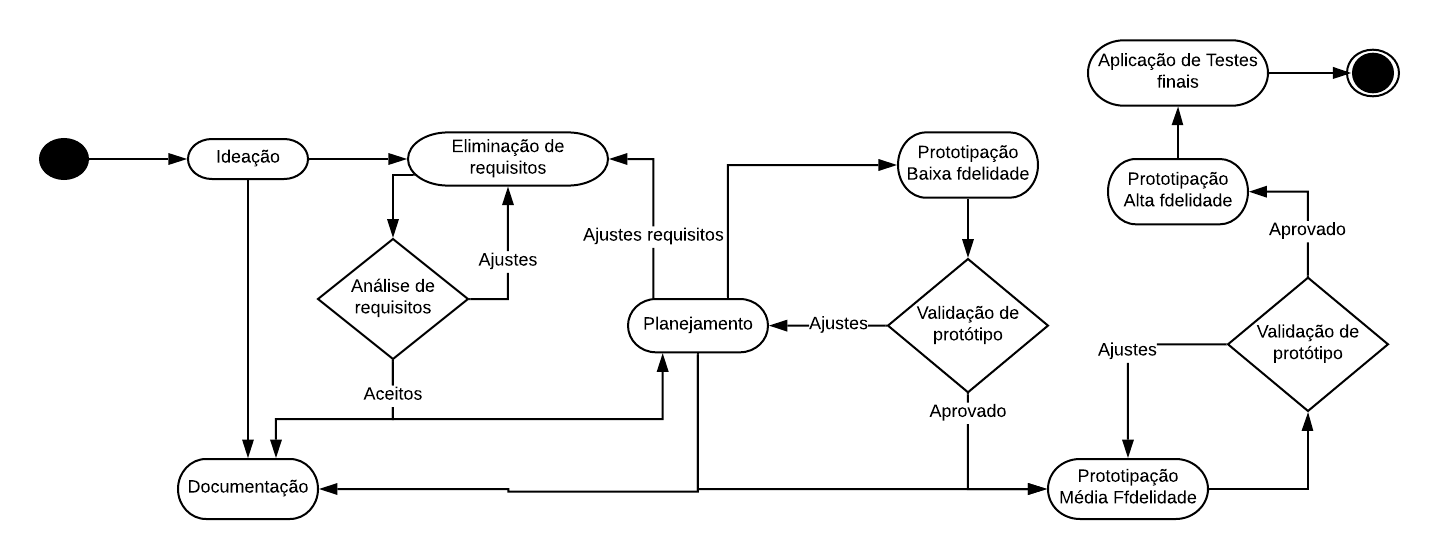
\includegraphics[width=1
			\textwidth]{imagens/diagramaDesenvolvimento.png}
			\caption{Diagrama de ciclo de software}
			\label{fig:diagram}
		\end{figure}
	
	\subsection{Ideação}
		Nesta etapa foram concebidas as primeiras ideias do jogo pela turma de professores Sateré Mawé, incluindo juntamente a identificação dos principais elementos e características da ferramenta, bem como o formato de sua \textit{gameplay} e mecânicas, além de fazer um rascunho inicial da proposta visual do jogo. Para tanto, utilizou-se de \textit{Brainstorns} para a criação de um ambiente para o compartilhamento de ideias entre o grupo de professores em suas comunidades para a definição da temática e o enredo do game. Afim de se estabelecer um referencial para o desenvolvimento do game, foi realizado uma busca por softwares similares e, dentre eles destaca-se jogos Trivia, por possuírem uma mecânica simples casual.     
	 
	\subsection{Elicitação de requisitos}
		Foram levantados os requisitos para o desenvolvimento do jogos, entre eles os requisitos funcionais e não funcionais, além dos aspectos pedagógicos e teoria cognitiva da aprendizagem.
	\subsection{Análise de requisitos}
		nesta etapa os requisitos foram analisados gerando as funcionalidades e restrições. Foram necessárias novas discussões que resultaram em novos requisitos e adaptações dos requisitos anteriores.
		
	\subsection{Planejamento}
		Durante esta fase foi realizada uma adaptação do \textit{Game Design Document} (GDD). Nele são apresentadas informações detalhadas do jogo, tais como: descrição de elementos da \textit{gameplay} e mecânicas, características das fases, controles do jogador, sons e efeitos sonoros no ambiente, detalhes do \textit{heads-up display} (HUD), entre outras.
	
	\subsection{Protótipo de Baixa Fidelidade}
		Conhecidos como as primeiras rasuras dos jogos, s˜ao normalmente construídos com materiais bem diferentes da versão final, de forma simples e clara. Este tem por objetivo demonstrar a ideia inicial do jogo, sendo considerado de fundamental importância nos estágios iniciais do desenvolvimento, pois trazem suporte `a busca de alternativas de design e ideias.
	
	\subsection{Protótipo de Média Fidelidade}
		O protótipo de média fidelidade seguiu as diretrizes presentes no GDD durante a implementação do jogo, executando conforme informações descritas na documentação. Nessa etapa foi utilizada a \textit{engine} \textit{Construct 2} para a implementação das primeira versões digitais da ferramenta.
	
	\subsection{Protótipo de Alta Fidelidade}
		O protótipo de alta fidelidade é a concepção que mais se assemelha com o produto que se pretende desenvolver, bem como consiste na implementação de melhorias no jogo. Nele estão implementadas todas as funções e alterações descritas na documentação e observadas nos testes iniciais de GameFlow, Rogers (2014). Para esta etapa empregou-se a engine \textit{Unity 3D}.
	
	\subsection{Validação de protótipo}
		A cada fim das etapas de protótipo de baixa, média e alta fidelidade, o aplicativo é avaliado para verificar se as funcionalidades implementadas estão de acordo com os requisitos definidos. A validação após protótipo de baixa e média fidelidade é realizada pelos desenvolvedores. Após o protótipo de alta fidelidade é realizada a avaliação das interfaces utilizando o Teste de Usabilidade de Nielsen \cite{nielsen1994usability} que também foi executado pelos desenvolvedores. 
		
	\subsection{Aplicação de testes finais}
		Nesta etapa são realizados testes com o usuário. O aplicativo proposto é validado com os usuários finais utilizando o teste MEGA+KIDS \cite{von2018meega+}, cujo objetivo é avaliar jogos com propósito educacional para aprendizagem de conceitos relacionados à computação.
		
	\subsection{Documentação}
		Durante todas as etapas do processo de desenvolvimento são gerados artefatos de documentação, entre eles o GDD.
		
	\section{Apresentação do Software}
		O Sehay etiat Wemaharap é um software educacional de gênero puzzle, com estilo top-dow, tendo como objetivo estimular e conservar o uso da língua materna Sateré Mawé dentre e fora das comunidades nativas por intermédio da resolução de problemas lógicos dispostos no
		game.
		
		No link é possível assistir ao vídeo demonstrativo do jogo: \textit{(https://www.youtube.com/watch?v=3ssmG7iYwOs)}.O desenvolvimento do aplicativo deu-se de acordo com o processo descrito a
		seguir representado na Figura \ref{fig:fluxoTela}.
	
		\begin{figure}[htb]
			\centering
			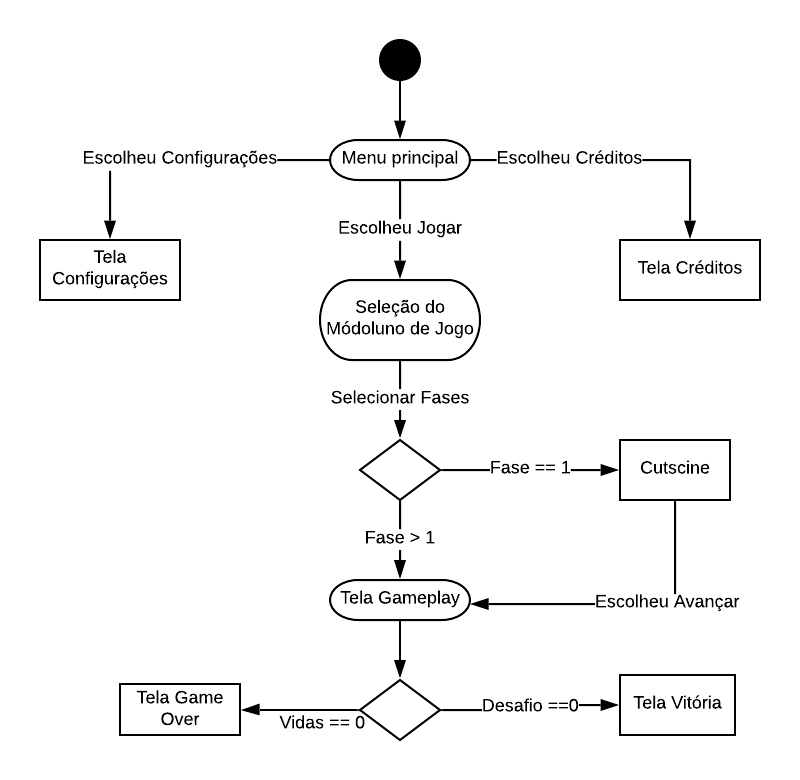
\includegraphics[width=.6\textwidth]{imagens/diag_fluxo_tela.png}
			\caption{Diagrama de fluxo de tela}
			\label{fig:fluxoTela}
		\end{figure}

	\subsection{Conceito do Jogo}
		Sehay etiat Wemaharap) é um jogo voltado para aprendizado da língua Sateré-Mawé, desenvolvido tanto para os que pertencem ao povo Sateré-Mawé quanto para quem possui o desejo de iniciar o aprendizado nela. Possui características que remetem a outros jogos por possuir estrutura clássica de jogos já conhecidos, assim também como uma elevada carga lógica.
		
		Atualmente conta com dois mini games bastante conhecidos que são subdivididos em três fases cada. O primeiro é o At'puenti (jogo da memoria), um clássico jogo da memória que possui alguns dos objetos tradicionais encontrados na cultura Sateré com suas respectivas palavas associadas. Em seguida encontra-se o game Sehay Wa’apopynug (palavras cruzadas), também fazendo uso da associação de objetos tradicionais e suas escritas utilizando em sua gameplay palavras totalmente em Sateré Mawé relacionadas a fauna e flora da cultura.    
		
	
	\subsection{Mecânica do Jogo}
\begin{figure}[!htb]
	\centering
	\minipage{0.31\textwidth}
	\includegraphics[width=\linewidth]{img/menu.png}
	\caption{Tela de Menu}\label{fig:menu}
	\endminipage \hspace{0.5cm}
	\minipage{0.31\textwidth}
	\includegraphics[width=\linewidth]{img/creditos.png}
	\caption{Tela de Vitoria}\label{fig:creditos}
	\endminipage
\end{figure}
		Ao iniciar o jogo o usuário deve escolher um dos níveis existente que aparecem logo após a tela de abertura e em seguida escolher uma das fases do nível. Cada fase tem um grau de dificuldade maior em relação a anterior, com a finalidade de instigar o jogador a jogar cada vez mais. Em toda fase há um determinado tempo que vai estabelecer o nível da fase, ou seja, quanto maior o tempo maior a dificuldade da fase. Essa conexão deixa a fase mais elaborada e cria um ambiente passível de vitória, mesmo com a dificuldade. 
		
		No primeiro mine game, será apresentado ao usuário uma série de peças com figuras e seus respectivos nomes em Sateré-Mawé, elas possuem pares, após mostradas são viradas para baixo. O jogador escolhe duas peças, caso sejam iguais são desviradas, caso contrario voltam ao estado anterior.
		
		No segundo game, os objetos estarão dispersas pela tela com seus respectivos campos para o preenchimento correto da parada, caso a letra escolhida pelo jogador não corresponder a string (nome) do objeto em questão, no decorrer de 2 segundos ela sera apagada, esperando para que o objeto seja escrito corretamente. Ao finalizar do tempo de cada fase, ou do da finalização da mesma, o jogador irar conquistar estrelas de acordo com seu progresso em cada uma das fases do jogo.   
		
		
	\subsection{Descrição das telas do jogo}
		Após o início do jogo, a tela de Menu inicial Figura \ref{fig:menu} dispõe do nome do jogo e, botões de iniciar e créditos. Clicando no ícone de Créditos Figura \ref{fig:creditos}, um pequeno pop-up exibirá informações sobre o desenvolvimento do game, onde ele foi desenvolvido e quais laboratórios de pesquisa e desenvolvimento estão envolvidos. Na Figura \ref{fig:jogos} são apresentadas as opções de mini games, logo em seguida, após a escolha do jogo (Figura \ref{fig:fases}), o usuário é direcionado para a tela de seleção de fases disponíveis para cada um dos desafios propostos.
	
	\begin{figure}[!htb]
		\centering
		\minipage{0.31\textwidth}
		\includegraphics[width=\linewidth]{img/selecNivel.png}
		\caption{Tela de Seleção de Jogos}\label{fig:jogos}
		\endminipage \hspace{0.5cm}
		\minipage{0.31\textwidth}
		\includegraphics[width=\linewidth]{img/selectFases.png}
		\caption{Tela de Seleção de Fases}\label{fig:fases}
		\endminipage
	\end{figure}
		
		Na Figura \ref{fig:exampleFig6} apresenta a tela de gameplay do primeiro mini game, que consiste em encontrar as palavras corretas para cada objeto. A Figura \ref{fig:exampleFig8} mostra a gameplay do segundo mini game. O usuário deve identificar o nome correspondente para cada objeto/animal encontrado na fase.
	
		\begin{figure}[!htb]
			\minipage{0.31\textwidth}
			\includegraphics[width=\linewidth]{img/memoryGame2.png}
			\caption{Jogo da Memoria}\label{fig:exampleFig6}
			\endminipage\hfill
			\minipage{0.31\textwidth}
			\includegraphics[width=\linewidth]{img/memoryGame.png}
			\caption{Jogo da Memoria fase 2}\label{fig:exampleFig7}
			\endminipage\hspace{0.4cm}%\hfill
			\minipage{0.31\textwidth}%
			\includegraphics[width=\linewidth]{img/palavraCruzadas.png}
			\caption{Palavras Cruzadas}\label{fig:exampleFig8}
			\endminipage
		\end{figure}
	
		Nas figuras \ref{fig:exampleFig11} e \ref{fig:feed} respectivamente, mostram as telas de pause (Figura \ref{fig:exampleFig11}) possuindo duas opções disponíveis: Jogar novamente e voltar ao menu inicial. O usuário pode acessar a esta tela em todos os níveis, representado pela figura anterior através do ícone no canto superior direito, dispondo das opções de voltar ao menu, ir para tela de seleção de fases ou voltar ao jogo. A próxima figura representa a tela de \textit{feedback} das pontuações conquistadas pelo jogador, sendo representado pela quantidade de estrelas obtidas. Ao completar cada faze dos jogos disponíveis, o jogador terá as opções de jogar o nível anterior, voltar ao menu inicial e ir para tela de seleção de fases (Figura \ref{fig:exampleFig12}).
		
		\begin{figure}[!htb]
			\centering
			\minipage{0.31\textwidth}
			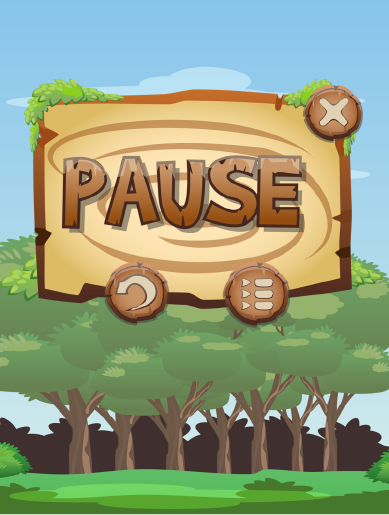
\includegraphics[width=\linewidth]{img/pause.png}
			\caption{Tela de Pause}\label{fig:exampleFig11}
			\endminipage \hspace{0.5cm}
			\minipage{0.31\textwidth}
			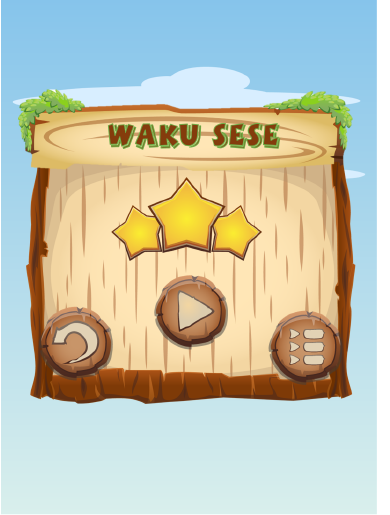
\includegraphics[width=\linewidth]{img/vitoria.png}
			\caption{Tela de Vitoria}\label{fig:feed}
			\endminipage
		\end{figure}
		
		
		\section{Considerações Finais}
			O Jogo demonstra ser uma ferramenta lúdica para o processo de aprendizagem da língua Sateré Mawé, visto que com ele o jogador entra em contato com a escrita da língua utilizando suas habilidades para resolução de problemas em um ambiente gameficado. O que viabiliza a difusão não apenas para quem fala a língua, mas também para os que ainda não tiveram contato com ela. Com o objetivo de analisar os níveis de imersão e diversão do game, serão utilizados os métodos Game Flow, que buscam aplicar heurísticas quanto a usabilidade do jogador. Futuramente pretende-se desenvolver uma nova versão na \textit{engine} Unity 3D com novos níveis, como o de expressões gramaticais em Sateré-Mawé.

	\bibliographystyle{sbc}
	\bibliography{sbc-template}

\end{document}
